\documentclass[a4paper, oneside]{csthesis}

\usepackage{etex}
\reserveinserts{28}

% package to be able to use special characters
\usepackage[utf8]{inputenc}

% Sophisticated math package
\usepackage{amsmath}

% Special symbols
\usepackage{amssymb}

\usepackage{siunitx}

% nicely render theorems and proofs
\usepackage[standard,thmmarks,amsmath]{ntheorem}

\usepackage{graphicx}

% package to format pseudo-code. Check the package documentation.
% http://ctan.org/pkg/listings
\usepackage{algorithmic}
\usepackage{algorithm}

% awesome code highlighting and coloring for many languages
% http://en.wikibooks.org/wiki/LaTeX/Packages/Listings
\usepackage{listings}
\lstset{language=Java}

% Provides \xspace command that evaluates to a space if the next character in the source is a blank and
% no space if next character is no blank. Useful in command definitions.
\usepackage{xspace}

% Provides a more flexible tabular environment
\usepackage{tabularx}

% Enables the use of the H location specifier for float environments that puts the float exactly where it is located in the source.
\usepackage{float}

% Enables the use of colours
\usepackage{color}

\usepackage{paralist}

% nice string commands
\usepackage{xstring}

\usepackage{colortbl}
\usepackage[table]{xcolor}

% wide tables
\usepackage{adjustbox}

\definecolor{DarkGray}{gray}{0.7}
\definecolor{MiddleGray}{gray}{0.8}
\definecolor{Gray}{gray}{0.9}

\definecolor{darkblue}{rgb}{0,0,.5}
% Enables clickable links in the PDF and additional PDF specific configuration options.
\usepackage[
            colorlinks=true,
            linkcolor=darkblue, urlcolor=darkblue, citecolor=darkblue,
						raiselinks=true,
            bookmarks=true,
            bookmarksopenlevel=1,
            bookmarksopen=true,
            bookmarksnumbered=true,
            hyperindex=true,
            plainpages=false,
            pdfpagelabels=true,
            pdfstartview=FitH,
            pdfstartpage=1,
            pdfpagelayout=OneColumn
            ]{hyperref}

% Provides a highly configurable way to create references inside the document and automatically prefix
% the number reference by fig./eq./chapter and so on. You only have to use \cref{label} or \Cref{label}
% to obtain "Lemma 4.1" or "Corollary 4.1" etc., depending on the label. See an example in the proof
% of the first theorem or check the documentation of the package for further information.
\usepackage[noabbrev]{cleveref}


% awesome figure placment
\usepackage{subfigure}

% Load own command definitions, a few helpful ones are already defined there.

% This alters the numbering of theorems and lemmas.
\theoremsymbol{\ensuremath{\scriptstyle \Diamond}}
\renewtheorem{theorem}{Theorem}[chapter]
\renewtheorem{lemma}[theorem]{Lemma}
\renewtheorem{corollary}[theorem]{Corollary}
\renewtheorem{definition}[theorem]{Definition}

% This creates a two new theorem-like environments
\theoremsymbol{}
\newtheorem{notation}[theorem]{Notation}
\theorembodyfont{}
\newtheorem*{problem}{Problem}

\crefname{algorithm}{algorithm}{algorithms}
\Crefname{algorithm}{Algorithm}{Algorithms}

% This changes the comment style of the "algorithmic" pseudocode package
\renewcommand\algorithmiccomment[1]{\hfill \small \(\triangleright\) #1}

% This creates four commands to leave annotations in your document
\newcommand{\TODO}[1]{\noindent {{\color{red}\fbox{\sffamily \bfseries TODO}} \sffamily #1}}
\newcommand{\FIXME}[1]{\noindent {{\color{green}\fbox{\sffamily \bfseries FIXME}} \sffamily #1}}
\newcommand{\CONSIDER}[1]{\noindent {{\color{blue}\fbox{\sffamily \bfseries CONSIDER}} \sffamily #1}}
\newcommand{\RW}[1]{\noindent \color{blue}#1}

% This creates a command to easily refer to websites as footnotes
\newcommand{\websource}[3]{\footnote{{#1\newline Available at: #2 [Accessed
#3]}}}

\newcommand\telesto{\textit{Telesto}}

\graphicspath{{figures/}}

% style whole rows in table
\usepackage{array}
\newcolumntype{$}{>{\global\let\currentrowstyle\relax}}
\newcolumntype{^}{>{\currentrowstyle}}
\newcommand{\rowstyle}[1]{\gdef\currentrowstyle{#1}%
  #1\ignorespaces
}


%%%%%%%%%%%%%%%%%%%%%%%%%%%%%%%%%%%%%%%%%%%%%%%%%%%%%%%%%%%%%%%%%%%%%%%%%%%%%%%%%%%%%%%%%%%%%%%%%
% DOCUMENT METADATA

\thesistype{Report Group 32}
\title{Telesto - A Distributed Message Passing System}

\author{Dominic Langenegger, Simon Marti}
\email{\{dominicl,simarti\}@student.ethz.ch}
\institute{Advanced Systems Lab 2013 \\[2pt]
Systems Group \\[2pt]
ETH Z\"urich}

% You can put in your own logo here "\includegraphics{...}" or just comment the command
% \logo{}

\supervisors{Markus Pilman\\[2pt] Prof.\ Dr.\ Gustavo Alonso}

% You can comment the following two commands if you don't need them
\keywords{}
%\categories{ACM categories go here.}

\date{November 15, 2013}

%%%%%%%%%%%%%%%%%%%%%%%%%%%%%%%%%%%%%%%%%%%%%%%%%%%%%%%%%%%%%%%%%%%%%%%%%%%%%%%%%%%%%%%%%%%%%%%%%

\begin{document}

\frontmatter
\maketitle % do not remove this line

\cleardoublepage

%\begin{acknowledgements}
%\end{acknowledgements}


\begin{abstract}
	This document describes \telesto, a distributed message passing system
	built as mandatory course work for the course {\it Advanced Systems Lab} at ETH
	Zurich in autumn semester 2013.
	
    After a short introduction, we describe the detailed architecture of the
    system and share some important implementation aspects before presenting
    various measurements on the running system that show stability, scalability
    and performance under different configurations. The measurements are
    discussed in detail and associated with the architecture in order to
    identify bottlenecks with respect to multiple performance metrics.
    
    A final conclusion summarizes our experience and learnings out of the whole
    project.

\end{abstract}

\tableofcontents

\mainmatter % do not remove this line

% Start writing here
\chapter{Introduction}
	For the Advanced Systems Lab course at ETH Zurich, students (in groups of two)
	have to build their own distributed message passing system following a very
	openly formulated project description~\cite{asl:course-description} which
	describes the most important requirements.
	
	The requirements specify the basic architecture of the system and its
	minimal functionality, but a very large part of the actual design of the system
	is leaved to the students. This is actually very beneficial for them because for
	many of them it is the first time they build such a large system from scratch
	and it is very educational to encounter all possible problems and actually find
	solutions for them.
	
	While the first part of the project work is about building the actual
	system, the second part is all about experimentally evaluate the whole system
	in its key performance characteristics. This includes tasks like running
	stability and scalability tests but also finding optimal system and workload
	parameters.
	
    In this second part, the task is not only to measure certain characteristics but
    also to learn how they arise and why the system behaves like it does.
	
	This report summarizes the entire project work during the design,
	implementation and evaluation of \telesto, the distributed message passing
	system built for the Advanced Systems Lab course in autumn semester 2013 by
	Dominic Langenegger and Simon Marti.
	
	
\section{Requirements}
    For the completeness of this document, we list the most important
    requirements of the distributed message passing system built (for details
    consult~\cite{asl:course-description} directly):
    
    \begin{itemize}
        \item The system consists of three tiers; i.e. a database, one or
        multiple middlewares and many clients.
        \item Clients only communicate with one middleware (and not with the
        database)
        \item The system lets clients manage queues containing messages by
        inserting and reading (while deleting) from them
        \item The whole system is built in {\it Java} using {\it PostgreSQL} as
        underlying database
        \item No external libraries exception for the {\it PostgreSQL JDBC}
        driver are allowed as part of the actual system. Also prohibited is the
        use of the {\it Java Persistence API (JPA)} and {\it Remote Method
        Invocation (RMI)}.
        \item The tests of the system should include at least one long running
        (\textgreater 2h) trace and many micro benchmarks analyzing separate
        parts of a messages way through the system. 
        \item Tests have to be repeated often enough to achieve statistical
        significance for the results
    \end{itemize}

    The project description contains various hints on how the system could be
    built in order to achieve a state of the art implementation that has good
    performance and is easy to evaluate during the testing phase.

\chapter{Goals}
    The goals for building \telesto{} was clearly producing a fast and very
    performant system with high scalability and stability. We especially put
    emphasis on creating an efficient way to communicate between client and
    the middleware using a lightweight packet format and capable request
    handling system.

	After an initial design phase we came up with a system supporting push based
	communication and complex caching on middlewares. We realized at the latest
	when a short {\it FAQ}~\footnote{Frequently Asked Questions} was published
	saying that we should build a pull based system, that our architecture was way
	too complex and can be replaced by a simpler, more transparent design.
	
	Out of this experience our aim to build a fast system shifted more to a system
	that is not only fast but also easy to test and understand in its details. Only
	with this in mind during implementation it is feasible to actually test the
	system in enough detail to be able to understand and correctly interpret the
	results.
	
	In the end we clearly wanted to analyze and identify the bottlenecks in
	\telesto{} with respect to various performance metrics.
	
\chapter{Architecture}
    This chapter explains the basic architecture of \telesto{} explaining how each
    part of the system works and how they communicate together.
    \Cref{ch:implementation} gives a more detailed insight about how the
    implementation of some important component looks like.

    \telesto{} is a three tier system:
    \begin{description}
        \item[Database] \ \\
            A {\it PostgreSQL}~\websource{PostgreSQL
            Website}{http://www.postgresql.org/}{November 15, 2013} database storing the persistent state of the system
        \item[Middleware] \ \\
            The part that provides many clients simultaneously with services of
            the message passing system and stores all data in the database. This
            part can be easily replicated.
        \item[Client] \ \\
            Clients that pass and receive messages from the system by talking to
            one middleware instance.
    \end{description}

    \Cref{fig:telesto-architecture} shows a sample architecture diagram.
    It is important to note, that clients only talk to middlewares and only a
    middleware has direct access to the database.

    \begin{figure}[h]
        \centering
            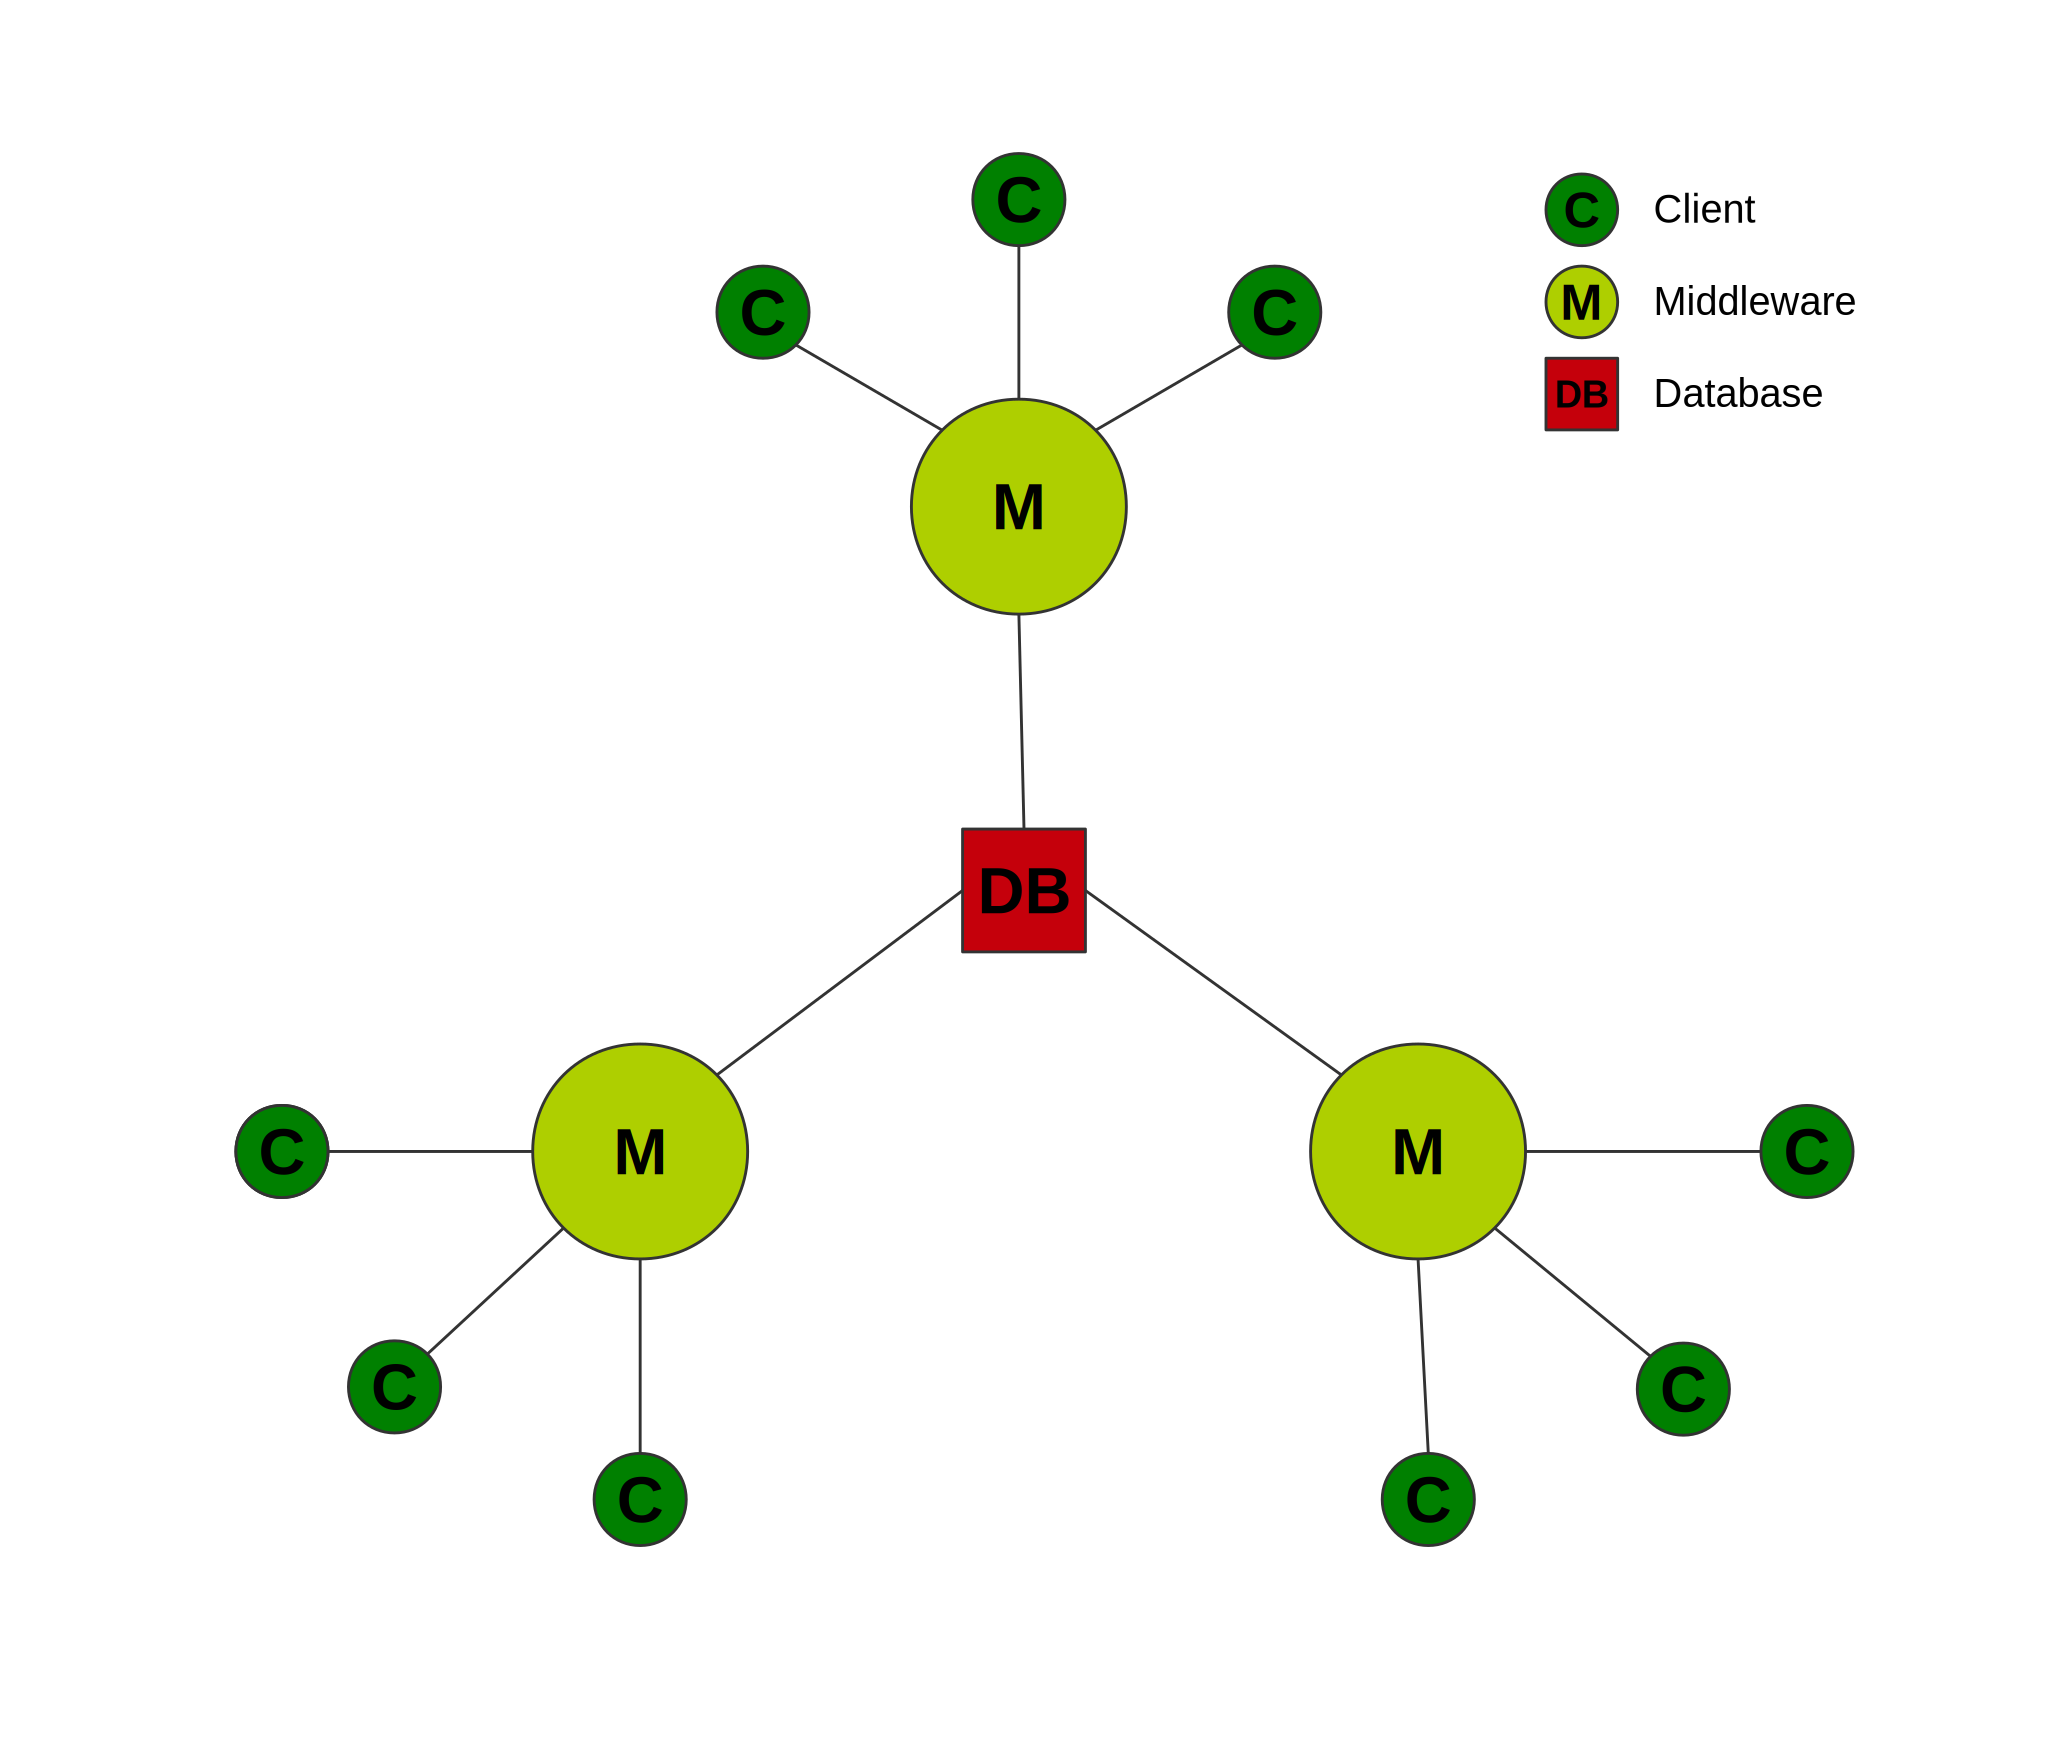
\includegraphics[width=0.9\textwidth]{architecture-new}
            \caption{Sample architecture diagram of \telesto{} with $3$
            middlewares each serving $3$ clients and one central database.}
            \label{fig:telesto-architecture}
    \end{figure}

\section{Database}
\label{sec:db}
    
    \telesto{} uses {\it PostgreSQL} as underlying database. It comes with a lot
    of features of which only a small subset are actually used by \telesto. The
    main directive for building the database was focusing on a simple and
    scalable design and using stored procedures to do all database interactions
    rather than prepared statements. The latter reduces the use of {\it SQL} in
    the middleware to an absolute minimum since only function calls have to be
    passed to the database.
    
\subsection{Entities}
    In \telesto{} there exist only three different entities:
    
    \begin{description}
    \item[Client] \ \\
        A client to the system identified by a unique name and client\_id.
        Clients have a certain mode indicating whether they are only allowed to
        read messages or also put new ones.
    \item[Queue] \ \\
        A queue that can contain multiple messages and is identified by a unique
        name and queue\_id
    \item[Message] \ \\
        A string message in exactly one queue with a client as sender, a
        potential receiver, a priority, a content string and, if the message is
        part of a request response interaction, a context. Additionally a
        timestamp is stored indicating when the message arrived in the system.
    \end{description}

    \begin{table}[t]
        \centering
        \rowcolors{1}{Gray}{white}
        \begin{tabular}{$l^c^r}
            \rowcolor{DarkGray}
            \rowstyle{\bfseries}
            Field name & type & Description\\
            \hline
            client\_id & serial & primary key using sequence \\
            client\_name & varchar(255) & unique \\
            client\_mode & smallint & \\
        \end{tabular}
        \caption{Table {\tt clients}}
        \label{tbl:db-clients}
    \end{table}
    
    \begin{table}[t]
        \centering
        \rowcolors{1}{Gray}{white}
        \begin{tabular}{$l^c^r}
            \rowcolor{DarkGray}
            \rowstyle{\bfseries}
            Field name & type & Description\\
            \hline
            queue\_id & serial & primary key using sequence \\
            queue\_name & varchar(255) & unique \\
        \end{tabular}
        \caption{Table {\tt queues}}
        \label{tbl:db-queues}
    \end{table}
    
    \begin{table}[b]
        \centering
        \rowcolors{1}{Gray}{white}
        \begin{tabular}{$l^c^r}
            \rowcolor{DarkGray}
            \rowstyle{\bfseries}
            Field name & type & Description\\
            \hline
            message\_id & serial & primary key using sequence \\
            queue\_id & integer &  \\
            sender\_id & integer & \\
            receiver\_id & integer & \\
            context & integer & \\
            priority & smallint & between $1$ (lowest) and $10$ \\
            time\_of\_arrival & timestamp & set to {\tt now()} by default \\
            message & varchar(2000) & the actual message \\
        \end{tabular}
        \caption{Table {\tt messages}}
        \label{tbl:db-messages}
    \end{table}

    Each of this entities can directly be modeled into one database table each
    as shown in \cref{tbl:db-clients,tbl:db-queues,tbl:db-messages}.

    In order to create the tables we used {\it PgAdmin 3}\websource{pgAdmin
    Website}{http://www.pgadmin.org/}{November 15, 2013} on a local
    development database and used the backup function to create a dump which
    could be distributed to our testing environment.
    
    We deliberately pass on creating foreign key constraints on our tables
    because 
    \begin{inparaenum}[\itshape a\upshape)]
        \item we use table joins for just one operation (i.e. {\tt
        get\_active\_queues()}, see \cref{sec:stored-procedures}) which can also
        be handled by an index; 
        \item we don't need any actions on update or deletion except for the
        case when a queue is deleted, which can easily be handled individually;
        \item we are sure that we don't insert inconsistent data because data is
        never updated~\footnote{There is actually no support to change queue or
        client names. This could however be added while still not rendering this
        argument invalid because only id rather than name attributes would be
        used as foreign keys} and queue existence is checked on insert; and
        \item we support inserting messages for not (yet) existing clients by
        design because they may only register themself at a later point in time.
    \end{inparaenum}

\subsection{Indexes}
    The main actions on the database in \telesto{} are inserting messages and
    removing them (by reading them). Since reading messages supports some
    parameters (see \cref{tbl:query-params}), it is strongly recommended to use
    appropriate indexes on the affected tables. Additionally to the indexes
    specifically introduced to optimize the performance of a selection or
    sorting operation for message finding, there are primary keys indexed on
    every table which lower the cost of getting entries directly by their id.
    
\begin{table}[t]
    \centering
    
    \begin{adjustbox}{center}
        \rowcolors{1}{Gray}{white}
        \begin{tabular}{$l^c^c^p{5cm}}
            \rowcolor{DarkGray}
            \rowstyle{\bfseries}
            Parameter & affected fields & required & Description\\
            \hline
            queue\_id & queue\_id & X &  \\
            receiver\_id & receiver\_id & X & matches if either {\tt null} or own
            client\_id \\
            sender\_id & sender\_id &  &  \\
            context & context &  & to identify responses \\
            mode & priority, time\_of\_arrival & X & one of both used for ordering
            \\
            
        \end{tabular}
    \end{adjustbox}
    \caption{Parameters of a message query}
    \label{tbl:query-params}
\end{table}

    Based on the data from \cref{tbl:query-params} we decided only use
    multi-column indexes for the table {\tt messages} that always include the
    {\tt receiver\_id} as first part and the {\tt queue\_id} as second. The {\tt
    receiver\_id} is either an integer value or {\tt null}. In both cases the
    query executor should be able to use the second part, namely the {\tt
    queue\_id} which is always present. The details of each separate index are
    listed below:
    
    \begin{description}
    \item[receiver\_id, queue\_id, priority] \ \\
        For a query by priority and without specified sender
    \item[receiver\_id, queue\_id, priority, sender] \ \\
        For a query by priority with specified sender
    \item[receiver\_id, queue\_id, time\_of\_arrival] \ \\
        For a query by time without specified sender
    \item[receiver\_id, queue\_id, time\_of\_arrival, sender] \ \\
        For a query by time with specified sender
    \end{description}

\subsection{Stored Procedures}
\label{sec:stored-procedures}

    As mentioned above, all database interaction is done using stored
    procedures\websource{PostgreSQL 9.3 
    Documentation: SQL Procedural Language
    }{http://www.postgresql.org/docs/9.3/static/plpgsql.html}{November 15,
    2013}\websource{PostgreSQL 9.3 Documentation: CREATE
    FUNCTION}{http://www.postgresql.org/docs/9.3/static/sql-createfunction.html}{November
    15, 2013}. For most of the database functions we used the standard {\it SQL}
    language syntax rather than the special {\it PL/pgSQL} language because the
    simple version serves almost all our requirements and it is often possible
    to write very easy queries in a very simple way. We however did not test if
    queries would run faster using {\it PL/pgSQL} because of the additional
    options {\it PostgreSQL} offers for these stored
    procedures.\websource{Advantages of Using PL/pgSQL in the official
    documentation
    }{http://www.postgresql.org/docs/9.3/static/plpgsql-overview.html\#PLPGSQL-ADVANTAGES}{November 15, 2013}

    \Cref{tbl:procedures} lists all implemented stored procedures in
    the database of \telesto.
    They very directly resemble the methods supported by our network protocol
    (see \cref{sec:protocol}) which means there is not much logic required on
    the middleware in order to execute a query on the database given a request
    packet.
    
    To simplify the database abstraction in the middleware we tried to produce
    very consistent return values. All functions either return tables of Queues,
    Messages, Clients, a set of integers or single integers. (where many are
    constrained to a single entry) For error handling, unique constraint violations are detected
    by the middleware and both {\tt put\_message} and {\tt put\_messages} return
    the {\tt queue\_ids} of the queues successfully inserted to (an id might be
    missing if the queue did not exist). Like this, errors from the database can
    be transformed into an appropriate {\tt ErrorPacket} as introduced in the
    next section.

\begin{table}[hp]
    \centering
    
    \begin{adjustbox}{center}
        \rowcolors{1}{Gray}{white}
        \begin{tabular}{$l^l^c^p{5cm}}
            \rowcolor{DarkGray}
            \rowstyle{\bfseries}
            Name & Parameters & Return Value & Description\\
            \hline

            \rowcolor{MiddleGray}
            \multicolumn{4}{c}{Client Manipulation} \\
            \hline
            request\_id & 
            \parbox[t]{2.5cm}{client\_name,\\ mode} 
            & client\_id & create
            a new client \\
            identify & client\_id & Client & identify a client \\
            delete\_client & client\_id & client\_id & delete a client \\
            
            \hline
            \rowcolor{MiddleGray}
            \multicolumn{4}{c}{Queue Manipulation} \\
            \hline
            create\_queue & queue\_name & Queue & creates a new queue \\
            delete\_queue & queue\_id & queue\_id & delete a queue \\
            get\_queue\_id & queue\_name & Queue & get queue by name \\
            get\_queue\_name & queue\_id & Queue & get queue by id\\
            list\_queues &  & array[Queue] & get all queues \\
            
            get\_active\_queues & client\_id & array[Queue] & get all queues with
            messages for the given client \\
            get\_messages\_from\_queue & queue\_id & array[Message] & get all
            message in a queue \\
            
            \hline
            \rowcolor{MiddleGray}
            \multicolumn{4}{c}{Message Manipulation} \\
            \hline
            put\_message & 
            \parbox[t]{2.5cm}{queue\_id,\\ sender\_id,\\ receiver\_id,\\
            context,\\
            priority,\\ message}
             & queue\_id & insert message and return queue
            \\
            
            put\_messages & 
            \parbox[t]{2.5cm}{array[queue\_id],\\ sender\_id,\\ receiver\_id,\\
            context,\\
            priority,\\ message}
             & array[queue\_id] & insert messages in multiple queues and return
             queues
            \\
            
            read\_message\_by\_priority & 
            \parbox[t]{2.5cm}{queue\_id,\\ sender\_id,\\ receiver\_id}
             & Message & get a message by priority
            \\
            
            read\_message\_by\_timestamp & 
            \parbox[t]{2.5cm}{queue\_id,\\ sender\_id,\\ receiver\_id}
             & Message & get a message by timestamp
            \\
            
            read\_response\_message & 
            \parbox[t]{2.5cm}{queue\_id,\\ receiver\_id,\\ context}
             & Message & get a message by receiver and context
            \\
            
            
            
        \end{tabular}
    \end{adjustbox}
    \caption{Parameters of a message query}
    \label{tbl:procedures}
\end{table}

\section{Network Protocol}
\label{sec:protocol}

    In order to achieve high throughput and low latency, it is essential to have
    a lightweight communication protocol as a foundation. \telesto{} uses a binary
    protocol based on TCP to do all the communication between clients and
    middlewares. Connections to the database are handled by the {\it PostgreSQL
    JDBC Driver}~\websource{PostgreSQL JDBC
    Driver}{http://jdbc.postgresql.org/}{November 15, 2013} which is based on
    TCP as well but isn't part of \telesto{} itself. This section gives insight
    about the network protocol introduced by \telesto{} for the communication
    between clients and middleware.
    
    A middleware offers a certain set of services (i.e methods) to the clients,
    like putting a message in a queue or reading a message from a queue. Every
    such method is identified by a special {\tt method id}. All method calls and
    responses are grouped into one \telesto{} packet consisting of four parts:
    \begin{description}
    \item[length] \ \\
        The length of the entire packet in bytes. This value is sent as a {\tt
        short} type integer which allows values of up to $32,768$. This limits
        the packet size, which is fine since the maximum supported message size
        is $2000$ characters and all other fields are a lot smaller. Only the
        method to read all messages from a queue might (in rare cases) try to
        serve more data which would then fail.
    \item[method id] \ \\
        A {\tt short} containing the method id in order to identify the service
        requested and how to interpret the payload.
    \item[client packet\_id] \ \\
        An id that is set by the client and repeated by the middleware in the
        associated response in order to identify which request yielded which response.
    \item[payload] \ \\
        The varying length payload containing all the arguments of the method
        call or the structured response data.
    \end{description}
    
     Figure \TODO{add
    protocol figure} shows the basic structure of such a packet.
    
    Besides a packet for each method call, there is one for the according
    response if applicable and two additional packets named {\tt SuccessPacket}
    and {\tt ErrorPacket} to indicate a successful call of a method with no
    return value or an error during execution respectively.
    
    By convention the {\tt packet id} for a response is always higher by one
    than the according request. A complete list of the currently supported methods and
    their parameters is shown in \cref{tbl:packets}.
    
    \begin{table}[hp]
        \centering
        \rowcolors{1}{Gray}{white}
        \begin{tabular}{$l^c^r}
            \rowcolor{DarkGray}
            \rowstyle{\bfseries}
            Packet & method\_id & payload\\
            \hline
            Ping & 0x01 & \\
            Pong & 0x02 & \\
            Success & 0x03 & \\
            Error & $0x05$ & error\_type, error\_string \\
            \hline
            \rowcolor{MiddleGray}
            \multicolumn{3}{c}{Client Manipulation} \\
            \hline
            RegisterClient & 0x11 & client\_name, mode\\
            RegisterClientResponse & 0x12 & client\_id\\
            IdentifyClient & 0x13 & client\_id\\
            IdentifyClientResponse & 0x14 & mode, client\_name\\
            DeleteClient & 0x15 & client\_id\\
            \hline
            \rowcolor{MiddleGray}
            \multicolumn{3}{c}{Queue Manipulation} \\
            \hline
            CreateQueue & 0x21 & queue\_name\\
            CreateQueueResponse & 0x22 & queue\_id\\
            DeleteQueue & 0x23 & queue\_id\\
            GetQueueId & 0x25 & mode, queue\_name\\
            GetQueueIdResponse & 0x26 & queue\_id\\
            GetQueueName & 0x27 & queue\_id\\
            GetQueueNameResponse & 0x28 & queue\_name\\
            GetQueues & 0x29 & \\
            GetQueuesResponse & 0x2a & array[Queue]\\
            GetActiveQueues & 0x2b & \\
            GetActiveQueuesResponse & 0x2c & array[Queue]\\
            GetMessages & 0x2d & queue\_id\\
            GetMessagesResponse & 0x2e & array[Message]\\
            \hline
            \rowcolor{MiddleGray}
            \multicolumn{3}{c}{Message Manipulation} \\
            \hline
            PutMessage & 0x31 & Message, array[queue\_id]\\
            ReadMessage & 0x32 & queue\_id, sender\_id, mode\\
            ReadMessageResponse & 0x33 & array[Message]\\
            ReadResponse & 0x34 & queue\_id, context\\
        \end{tabular}
        \caption{Supported packets in \telesto. By convention an odd {\tt
        method\_id} indicates client to server communication while even values
        are server to client communication. Queue and Message objects in the
        payload include all fields stored in the database (see \cref{sec:db}).
        The {\tt mode} in the ReadMessage packet is used to indicate whether
        the oldest message or the one with the highest priority should be
        served.}
        \label{tbl:packets}
    \end{table}
    
    By using this lightweight binary packet format, the overall packet size is
    only slightly larger than a binary sequence of all input parameters of a
    method which is certainly a good prerequisite for handling high loads with
    many requests in short time. 
    %As seen in \cref{ch:evaluation}, the load on the network was never a
    % problem during performance tests.


\section{Middleware}

    The middleware is the core part of \telesto{} as it serves incoming request
    from clients in a highly efficient manner. The tasks arising can be split in
    $4$ parts:
    
    \begin{enumerate}
        \item Handling incoming connections and data
        \item Parsing the request packet
        \item Executing the according database action
        \item Sending back a response
    \end{enumerate}

    Using asynchronous Java {\tt
    nio}\websource{Java
    Documentation:
    java.nio}{http://docs.oracle.com/javase/7/docs/api/java/nio/package-summary.html}{November
    15, 2013}, it is possible to handle a lot of concurrent connections to
    multiple clients simultaneously in an efficient manner. A single
    dispatcher thread handles new incoming connections and data by putting
    the clients into a FIFO queue which is continuously worked off by multiple
    worker threads. The actual parsing, database action and response sending is done by
    a worker rather than the dispatcher in order to reduce the load on the
    dispatcher.
    
    In order to interact with the database, a database connection pool is used
    with a limited number of connections. Workers can request a connection from
    this pool, execute their queries and then put the connection back for other
    workers to use.
    
    \Cref{fig:middleware} shows an overview of the three main parts in the
    middleware; namely the dispatcher, the worker threads and the database
    connection pool.
    
    It is important to note, that connections to clients are never closed by the
    middleware (unless on shutdown). This first improves the delay of the
    system because no new TCP connection establishment is necessary for each
    request and second it allows to store the client information together with
    the connection so it is never necessary to send the {\tt client\_id} to the
    middleware again after the initial identification. This is the reason, why
    every client is first only allowed to request a limited set of services
    because many of them require identification. These services are namely the
    client registration and identification, and the pinging system.

    \begin{figure}[ht]
        \centering
            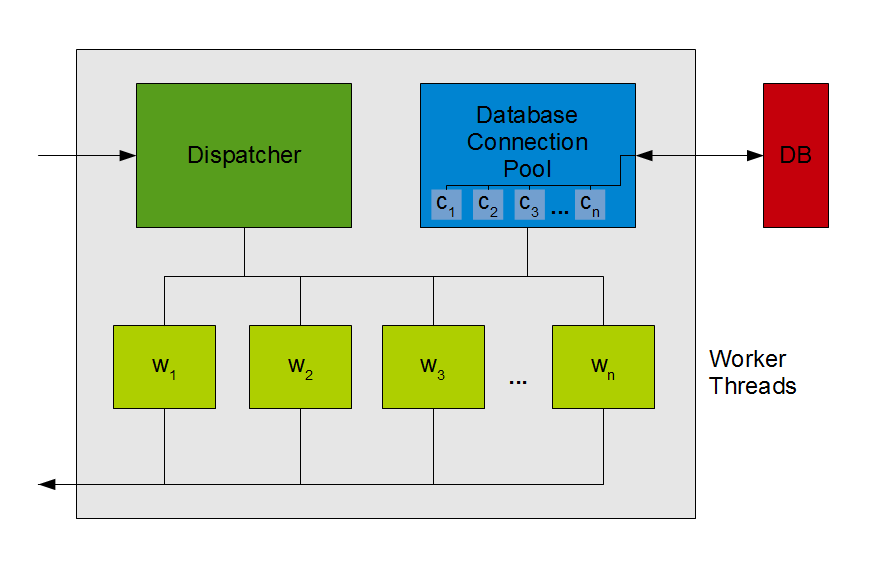
\includegraphics[width=0.9\textwidth]{middleware}
            \caption{Basic setup of a middleware instance including the
            dispatcher, multiple worker threads and a database connection pool.}
            \label{fig:middleware}
    \end{figure}


\section{Client}
    \telesto{} offers a simple interface for clients that want to use the system.
    The actual public Application Programming Interface (API) consists of one
    simple class {\tt TelestoClient} with all the offered functionality. It is
    as easy as creating a new instance and then start calling functions to
    actually use \telesto.
    
    By design, a client is only allowed to do further actions if he either
    registered itself as a new client or identified itself using his client id.
    This means, the first API call has to be to the {\tt connect()} or method
    supplying either an existing {\tt client\_id} or both a new name and the
    mode of the client. (or {\tt ping()} which is always allowed)
    
    The API works in a synchronous way and has some blocking functions that
    retry an operation with a certain (configurable) delay until successful. An
    example of this is requesting a message from a queue, which blocks until a
    message for the client is successfully read.
    
    It would be possible to actually build a client implementation that is
    asynchronous since the middleware and the used protocol support that
    feature. However we went without such an implementation as the testing of
    the system is in many cases much easier when using synchronous clients.
    

\chapter{Implementation}
\label{ch:implementation}
This chapter gives more detailed overview of some decisions made during the
implementation phase of \telesto. This is a good starting point before getting
involved with the code base of the system as it gives the necessary orientation
and overview.

The whole code base is organized into six java packages that resemble the
different parts of \telesto:

\begin{description}
\item[ch.ethz.syslab.telesto.client] \ \\
    The \telesto{} client including the API and multiple specific
    implementations for different tests in the subpackage {\tt test}.
\item[ch.ethz.syslab.telesto.common] \ \\
    All the parts that are shared between the middleware and the client
    implementation with for example model classes for all entities, the
    configuration and the protocol.
\item[ch.ethz.syslab.telesto.console] \ \\
    The implementation of the management console displaying all important
    information of the system.
\item[ch.ethz.syslab.telesto.profile] \ \\
    Classes specifically used for profiling and benchmark logging. These are
    used by both the client and the middleware.
\item[ch.ethz.syslab.telesto.server] \ \\
    The \telesto{} middleware with all database related functionality in the
    subpackage {\tt db}, the dispatcher and worker thread implementations in the
    subpackage {\tt network} and the protocol handlers in the subpackage {\tt
    controller}.
\item[ch.ethz.syslab.telesto.test] \ \\
    An extensive test suite containing jUnit tests for many different parts of
    the system.
\end{description}

We chose to develop \telesto{} using {\it Eclipse (Version 4.3.1
Kepler)}\websource{Eclipse website}{http://eclipse.org/}{November 15, 2013}
as integrated development environment (IDE) and {\it
git}\websource{Official git website}{http://git-scm.com/}{November 15, 2013}
with a (private) {\it Github}\websource{Github
website}{https://github.com/}{November 15, 2013} repository as version control
and source code management system.


\section{Networking}
    In order to make networking efficient and fast, it is essential that
    involved parts of the system are never a bottleneck to the entire system
    performance.
    
    The crucial part of this is optimizing the load on the dispatcher (i.e. an
    instance of the class {\tt ConnectionHandler}) and limiting the overhead of
    distributing the tasks over all the workers (i.e. instances of {\tt
    DataHandler}).
    This is why \telesto{} uses a {\tt ArrayBlockingQueue<Connection>} to manage incoming requests that can then be
    processed by worker threads in a first-in-first-out (FIFO) manner. Since
    this data structure is backed by a simple array, runtime for inserting and
    removing from the queue always stays $\mathcal{O}(1)$.
    
    The drawback of this implementation is that the queue has a limited size
    that is initially set and cannot be changed during execution.
    This however is not a problem because with the synchronous I/O in the
    clients, where they always wait for a response before requesting another
    service, the maximum number of connections in the queue should never
    actually grow larger than the number of clients. Therefore it is sufficient
    to ensure that the number of clients is always lower than the queue size.
    
    In a scenario where clients would asynchronously send many requests
    simultaneously or the number of clients is much higher than the queue size,
    it becomes possible, that the dispatcher becomes blocked when trying to put
    a connection into the queue because it is already full. If the system is
    expected to run under such circumstances, then it would be necessary to
    improve the implementation for this special workload e.g. by dynamically
    replacing the queue with an other larger one or by just rejecting all
    incoming requests while the queue is full.
    
    However in the settings where \telesto{} was tested in this was not critical
    and the chosen implementation proofed to be fast enough to never become a
    bottleneck to the whole system.
    
    
\subsection{Packet parsing}
    A special part of \telesto{} is its binary packet format (see
    \cref{sec:protocol}) which requires special handling of the incoming data
    for every method supported. For this purpose, the package {\tt
    ch.ethz.syslab.telesto.common.protocol}, contains one class for every packet
    with the following components (as specified in the abstract class {\tt
    Packet}):
    
    \begin{enumerate}
        \item All the parameters that are part of the packet as fields
        \item The method {\tt emit()} to write the fields to a {\tt
        ByteBuffer}
        \item The method {\tt parse()} to build a packet instance from
        a {\tt ByteBuffer}
    \end{enumerate}

    Because it is a rather ungrateful task to write about $30$ packet classes
    and according handlers that share many lines of code, we built an automated
    {\it Python}\websource{Python Website}{http://python.org/}{November 15, 2013}
    script to generate all packet and packet handling classes using {\it
    jinja2}\websource{Jinja2
    Documentation}{http://jinja.pocoo.org/docs/}{November 15, 2013} templates
    and a small configuration specifying what packets exist with what fields.
    
    The code for this tasks is available under {\tt tools/protocol/} with the
    packet specification in the source file {\tt messages.py}. The initial
    effort to build this small tool was very much worth it because it makes
    actually changing the protocol or the methods and implementation of a class
    very easy because all handler and packet classes can be regenerated using
    very little effort.
    
\subsection{Packet handling}
    Each worker parses incoming data using the static method {\tt
    create(ByteBuffer)} in the abstract {\tt Packet} class which creates an
    instance of the right packet class using the method id at the very beginning
    of the packet data and lets this instance's {\tt parse(ByteBuffer)} method
    handle the parsing of the individual fields.
    
    The built packet instance containing all information that was sent over
    the network is then handled by a {\tt ProtocolHandler} that contains a
    method {\tt handle()} that is overloaded to take every existing packet as
    input and returning a packet as response to be sent back to the client. This
    class is actually also generated by the above mentioned automated python
    script to contain all the necessary methods.
    
    For the overloading to correctly work with the dynamic typing and
    instantiation of the packet classes, it is necessary to use the visitor
    pattern on the packet classes to let them call the handle method for
    themself.
    
    \telesto contains two different implementations for the {\tt
    ProtocolHandler}:
    \begin{description}
    \item[ServerAuthenticationProtocolHandler] \ \\
        The protocol handler for all the packets that are allowed to send before
        authentication. An instance of this class is switched out by one of
        {\tt ServerProtocolHandler} as soon as authentication is completed.
    \item[ServerProtocolHandler] \ \\
        The actual protocol handler that handles all packets that are sent to a
        middleware instance. Each {\tt handle()} methods contains the necessary
        logic to query the database and build a response for the client.
    \end{description} 

    In order to handle packets that should not be sent to the server (i.e.
    response packets), the abstract {\tt ProtocolHandler} just throws an
    appropriate exception that is converted into an {\tt ErrorPacket} upon
    catching in the worker to notify the client of his misbehaving.

\section{Database}
    As explained in \cref{sec:db}, \telesto{} uses stored procedures for all
    database interaction. Using the {\it PostgreSQL JDBC} driver, it is rather
    easy to make calls to such a procedure but a lot of code lines goes into
    error handling, statement generation (i.e. setting parameters) and reading
    out the response data and build entity instances.
    
    This is why we built a heavy abstraction around the {\it JDBC} driver that
    is able to share most of the code and takes care of statement generation,
    error handling and directly returns appropriate entity objects (or lists) to
    be used in the response packets. Using this abstraction layer, it is
    possible to initiate all database action using a single line of code in the
    {\tt ProtocolHandler} implementation.
    
    As seen in \cref{sec:stored-procedures}, there are only five different
    return value types for all procedures:
    
    \begin{enumerate}
        \item Table of Clients
        \item Table of Queues
        \item Table of Messages
        \item Set of Integers
        \item Single Integer
    \end{enumerate}
    
    Therefore our abstraction contains an {\tt enum} in the package {\tt
    db.procedure} for each of the first three where all available stored
    procedure are enumerated according to their return value. Procedures
    returning integers are included in the {\tt enum} that best categorizes
    them.
    
    By offering a simple method on the {\tt Database} class (which does all
    database related work) for each of the above stated types, it is possible to
    directly return the according instances and control (to some extent) that
    only procedures really producing that output type can be called. The
    signature of such a function looks like this:
    
    \begin{center}
        {\tt public List<Message> callMessageProcedure(MessageProcedure proc,
        Object... arguments)}
    \end{center}

    Each {\tt enum} value contains the necessary information to assign the
    right types to the arguments, the return type and the name of the stored
    procedure in the database.
    
\subsection{Connection Pool}
    For the implementation of the database connection pool, \telesto{}
    completely relies on the {\it PostgreSQL JDBC} driver which
    offers a complete implementation in the {\tt
    PGPoolingDataSource}\websource{PGPoolingDataSource in the PostgreSQL JDBC
    driver documentation
    }{http://jdbc.postgresql.org/documentation/publicapi/org/postgresql/ds/PGPoolingDataSource.html}{November 15, 2013}
    class.


\section{Client}
    \Cref{tbl:client-api} shows a brief overview of the offered
    functionality by the \telesto{} client API. A more detailed description of
    each method is available inside the class {\tt
    ch.ethz.syslab.telesto.client.TelestoClient} as {\it
    javadoc}\websource{Oracle:
    How to Write Doc Comments for the Javadoc Tool
    }{http://www.oracle.com/technetwork/java/javase/documentation/index-137868.html}{November 15, 2013}.
    
    \begin{table}[p]
        \centering
        
        \begin{adjustbox}{center}
            \rowcolors{1}{Gray}{white}
            \begin{tabular}{$l^l^c^p{4cm}}
                \rowcolor{DarkGray}
                \rowstyle{\bfseries}
                Method & Parameters & Return Value & Description \\
                \hline
                \rowcolor{MiddleGray}
                \multicolumn{4}{c}{Setup} \\
                \hline
                
                ping & & round trip time & ping the middleware \\
                connect & 
                \parbox[t]{2.5cm}{clientName,\\ clientMode} & Client & connect
                to the middleware as new client  \\
                connect & clientId & Client & connect to the middleware as
                existing client \\
                
                \hline
                \rowcolor{MiddleGray}
                \multicolumn{4}{c}{Queues} \\
                \hline
                createQueue & queueName & Queue & create a new queue \\
                deleteQueue & queueId &  & delete a queue \\
                getQueueByName & queueName & Queue & get a queue by its name \\
                getQueueById & queueId & Queue & get a queue by its id \\
                getQueues &  & List\textless Queue\textgreater & get all queues \\
                getActiveQueues &  & List\textless Queue\textgreater & get all queues with messages
                for this client \\
                readMessages & queueId & List\textless Message\textgreater & get
                all messages from a queue
                \\
                
                \hline
                \rowcolor{MiddleGray}
                \multicolumn{4}{c}{Messages} \\
                \hline
                putMessage & Message &  & insert a new message \\
                putMessages & 
                \parbox[t]{2.5cm}{Message,\\ queueId[]} &  & insert a new
                message into multiple queues \\
                sendRequestResponseMessage & Message & Message & send request
                and retrieve response
                \\
                retrieveMessage & queueId & Message & get message from queue
                by priority \\
                retrieveMessage & 
                \parbox[t]{2.5cm}{queueId,\\ readMode} & Message & get message
                from queue by the indicated readMode
                \\
                retrieveMessage & 
                \parbox[t]{2.5cm}{queueId,\\ senderId,\\ readMode} & Message &
                get message from specific sender from queue by the indicated
                readMode
                \\
                retrieveMessage & 
                \parbox[t]{2.5cm}{queueId,\\ senderId,\\ readMode} & Message &
                get message from specific sender from queue by the indicated
                readMode
                \\
                
            \end{tabular}
        \end{adjustbox}
        \caption{Public methods on the {\tt TelestoClient} class. The class is
        also fully documented using {\it javadoc} in order to allow for
        easy usage.}
        \label{tbl:client-api}
    \end{table}
    
    The networking of the client is mostly shared with the one in the middleware
    but does not need any special {\tt ProtocolHandler} because it doesn't
    directly use any content of the response packets. Those are directly handled
    in the {\tt TelestoClient} where the returned packet is casted to the right
    response packet before the information is extracted and returned to the user
    calling the API function.

\section{Error Handling}
    Other than just handling errors within a single application, \telesto{} has
    to handle errors that occur in an other part of the system appropriately.
    This is the case if something goes wrong in the middleware which makes it
    necessary to inform the client that his request could not be executed. In
    order to do this, there exists a special {\tt ErrorPacket} (as introduced
    in \cref{sec:protocol}) that contains an error number and an error message.
    
    Possible error codes are stored in the enum {\tt ErrorType} and are listed
    in \cref{tbl:error-codes} together with a short description.
    
    \begin{table}[ht]
        \centering
        
        \begin{adjustbox}{center}
            \rowcolors{1}{Gray}{white}
            \begin{tabular}{$l^p{8cm}}
                \rowcolor{DarkGray}
                \rowstyle{\bfseries}
                ErrorType & Description \\
                \hline
                \rowcolor{MiddleGray}
                \multicolumn{2}{c}{Unexpected} \\
                \hline
                INTERNAL\_ERROR & A typically unexpected error \\
                IO\_ERROR & An error during network interaction \\
                
                \hline
                \rowcolor{MiddleGray}
                \multicolumn{2}{c}{Client Error} \\
                \hline
                UNEXPECTED\_PACKET & A packet that could not be handled was
                received
                \\
                UNIQUE\_CONSTRAINT & A unique constraint was violated \\
                QUEUE\_NAME\_NOT\_UNIQUE & The specified {\tt queue\_name} is
                not unique \\
                CLIENT\_NAME\_NOT\_UNIQUE & The specified {\tt client\_name} is
                not unique \\ 
                CLIENT\_NOT\_EXISTING & The specified client does not exist \\
                QUEUE\_NOT\_EXISTING & The specified queue does not exist \\
                REQUIRED\_PARAMETER\_MISSING & A required parameter in a packet
                is missing \\
                CLIENT\_MODE\_PERMISSION\_VIOLATION & The {\tt ClientMode}
                prohibits the use of the called service \\
                
                \hline
                \rowcolor{MiddleGray}
                \multicolumn{2}{c}{Client Notification} \\
                \hline
                
                NO\_ACTIVE\_QUEUES\_EXISTING & No queues contains messages for
                the client \\
                NO\_QUEUES\_EXISTING & There exist absolutely no queues \\
                NO\_MESSAGES\_IN\_QUEUE & There are no messages in the specified
                queue \\
                NO\_MESSAGES\_RETRIEVED & A receive query did not yield any
                messages \\
                
                
                
            \end{tabular}
        \end{adjustbox}
        \caption{Error codes in the system. Specified in the class {\tt
        ErrorType}.}
        \label{tbl:error-codes}
    \end{table}
    
    Additionally two special exceptions were introduced to handle errors within
    the system in a simple way:
    \begin{enumerate}
        \item {\tt ProcessingException} on the client
        \item {\tt PacketProcessingException} on the middleware
    \end{enumerate}
    Both exceptions allow to specify an {\tt ErrorType} and can include nested
    exceptions.
    
    When a {\tt PacketProcessingException} is thrown in the middleware, it is
    automatically caught and sent to the client in an {\tt ErrorPacket} where it
    is again processed into a {\tt ProcessingException} which is handled
    accordingly or thrown to the user.
    
\subsection{Logging}
    \telesto{} does not only have a solid error and exception system but also
    uses logging in many places to allow for deep investigation of possible
    problems. For this purpose we introduced the statically accessed {\tt Log}
    class that operates as a facade to {\tt java.util.logging}\websource{
    Java Documentation: java.util.logging
    }{http://docs.oracle.com/javase/7/docs/api/java/util/logging/package-summary.html}{
    November 15, 2013}
    . The use of
    the built in {\it Java} logging interface, allows to configure logging
    parameters in a very convenient and powerful way.

\section{Configuration}
    To configure client and middleware instances, \telesto{} uses both a
    configuration file and command line parameters. The following two sections
    briefly describe how both work.
    
\subsection{Configuration File}
    Both the client and the middleware use the same global {\tt
    config.properties} file to read the configuration for the current run. If no
    such file is present in the execution directory, then a default version is
    extracted from within the compiled {\tt .jar} file.
    
    This configuration file is a simple {\it Java Properties}
    file\websource{Java Documentation: java.util.Properties
    }{http://docs.oracle.com/javase/7/docs/api/java/util/Properties.html}{November
    15, 2013} containing parameters like the middleware address or database
    connection information. Details about these parameters and how they were
    varied over multiple tests, are explained in \cref{sec:parameters}.

\subsection{Command Line Parameters}
    Even if the code base is organized in a way that would allow building
    multiple {\tt .jar} files for client and middleware, we decided to just
    build one and use command line parameters in order to determine which part
    to start. This makes it more convenient to do tests because only one {\tt
    .jar} file has to be distributed over many machines.
   
    The first parameter always determines which tier should be started. The
    values ``MW'' and ``CL'' stand for middleware and client respectively.
    Only the client takes some additional arguments to control the following
    parameters:
    
    \begin{description}
    \item[name] The {\tt client\_name} to be used (registers new client)
    \item[id] The {\tt client\_id} (identifies as existing client)
    \item[test] An identifier for the test to run (see section
    \cref{sec:client-types})
    \end{description}

    These additional arguments are always supplied as key-value pairs separated
    by a space character. Of the name and the client id only one has to be
    specified.

\chapter{Evaluation and Analysis}
\label{ch:evaluation}
	This chapter gives an overview of the experiments conducted with \telesto{} and
	their results and implications.

\section{Setup}
	We conducted all experiments on the {\it Amazon Elastic Compute Cloud}\websource{Amazon EC2
    Website}{http://aws.amazon.com/ec2/}{November 15, 2013} (EC2).
    One large general purpose instance was used for each the database, the
    middleware and the clients.
    The experiments were controlled by a fourth instance which was allowed shell access on all of the
    other ones. All instances were placed on the same sub-network within {\it Amazon}'s network in order
    to minimize network latency.
    
    The experiments were controlled by a single configuration file which was
    automatically distributed by the controlling instance to the clients and the
    middleware for each test, using a {\tt bash} script.
    Given a number of these configuration files the controlling instance was
    able to run multiple experiments completely autonomous.
    
    The clients and the middleware are built to measure the duration of each phase a request goes
    through and write the results into a log file which is collected by the controlling instance
    and can then be processed.
    
\section{Client Types}
\label{sec:client-types}

    The system was tested using three different kind of clients to simulate a
    practical workload that includes multiple different applications of a
    message passing system:
    
    \begin{description}
    \item[One Way] \ \\
        These clients send a message containing a counter value to a random
        other client of the same type and then wait for a message for them. Upon
        receiving a message they increase the counter and again send it to a
        random other client. This was implemented using a single queue for all
        one way clients.
    \item[Request Response Pair] \ \\
        These clients act in pairs as client and server. They basically send
        messages back and forth between them both increasing a counter which is
        part of the message text. All these clients again use only one
        single queue.
    \item[Request Response Pool] \ \\
        Contrary to the clients acting in pairs, these clients act in two
        equally sized pools of clients and servers. Clients make a request which
        is answered by any client of the server pool. All requests and responses
        were stored in the same queue.
    \end{description}
    
    All tests described below were conducted using the distribution shown
    in~\cref{tbl:client-type-distribution}.

    \begin{table}[hp]
        \centering
        \rowcolors{1}{Gray}{white}
        \begin{tabular}{$l^c^r}
            \rowcolor{DarkGray}
            \rowstyle{\bfseries}
            Client Type & Fraction \\
            \hline
            One Way & $5/9$ \\
            Request Response Pair & $2/9$ \\
            Request Response Pool & $2/9$ \\
        \end{tabular}
        \caption{Client type distribution for all tests}
        \label{tbl:client-type-distribution}
    \end{table}

\newpage
\section{Parameters}
\label{sec:parameters}

	All experiments were run with the same basic parameters, save the ones being experimented on.
	Before each experiment the database was emptied to get consistent results.
	The default parameters are listed in \cref{tbl:parameters}.
	
	\begin{table}[hp]
        \centering
        \rowcolors{1}{Gray}{white}
        \begin{tabular}{$l^c^r}
            \rowcolor{DarkGray}
            \rowstyle{\bfseries}
            Parameter & Value\\
            \hline
            Running time & 10 minutes \\
            \hline
            \rowcolor{MiddleGray}
            \multicolumn{2}{c}{Client} \\
            \hline
            Number of instances & 90 \\
            Retry delay & 100ms \\
            Network buffer size & 32KB \\
            \hline
            \rowcolor{MiddleGray}
            \multicolumn{2}{c}{Middleware} \\
            \hline
            Number of instances & 1 \\
            Network buffer size & 32KB \\
            Worker pool size & 25 \\
            Database pool size & 25 \\            
        \end{tabular}
        \caption{Default parameters for experiments}
        \label{tbl:parameters}
    \end{table}

\section{Metrics}
	\begin{description}
		\item[Middleware response time] \ \\
		    Time the client waits for a response after sending a request to the server.
		\item[Packet parsing duration] \ \\
		    Time the middleware needs to parse a request from a client.
		\item[Database response time] \ \\
		    Time the middleware waits for a response from the database after making a request.
		\item[Packet emitting duration] \ \\
		    Time the middleware needs to construct and send a response to the client. 
		\item[Middleware worker downtime] \ \\
		    Time a worker instance of the middleware waits before receiving a client request to handle.
		\item[Packet throughput] \ \\
		    Number of network packets sent by the middleware.
		\item[Message throughput] \ \\
		    Number of messages successfully received by a client.
	\end{description}

\section{Experiments}
	The experiments were generally run for 10 or 5 minutes to make sure the relative confidence interval
	for a certainty of 95\% is alwasy lower than 5\%. We never experienced messages or packets being
	dropped during any of the conducted experiments.

\subsection{Stability}
	To measure the stability of our system we ran it with the default configuration for 2 hours without
	interruption. 

    \begin{figure}[ht]
    \centering
        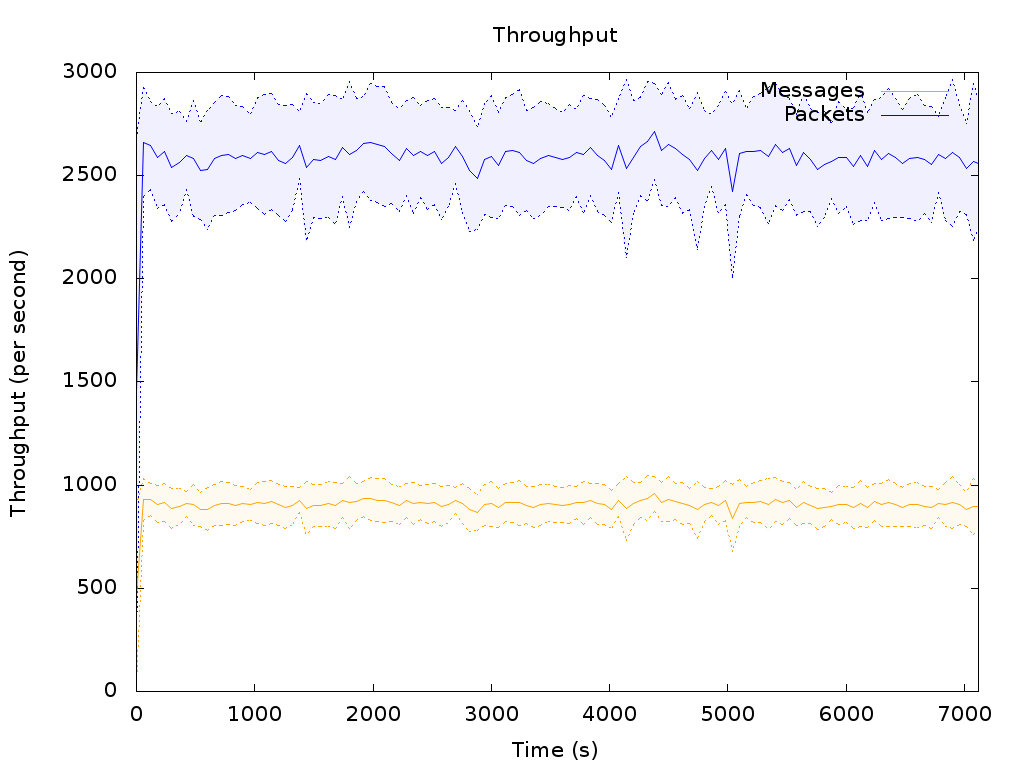
\includegraphics[width=0.9\textwidth]{graphs/throughput}
        \caption{Throughput measured every second and averaged over an interval of one minute.}
        \label{fig:throughput}
    \end{figure}

	\Cref{fig:throughput} shows the message and packet throughput as measured by the clients over time.
	The throughput was measured every second and averaged over the interval of one minute in the shown figure.
	
	It is clearly visible that our system is fairly stable over such a long period of time. The small variation
	seen especially in the packet throughput most likely originated in the unpredictable network environment
	of the {\it Amazon Cloud}. It is further visible that the packet throughput is roughly 3 times as
	big as the message throughput, meaning that only around one sixth of message requests by clients
	returned no messages.
    
    \begin{figure}[ht]
    \centering
        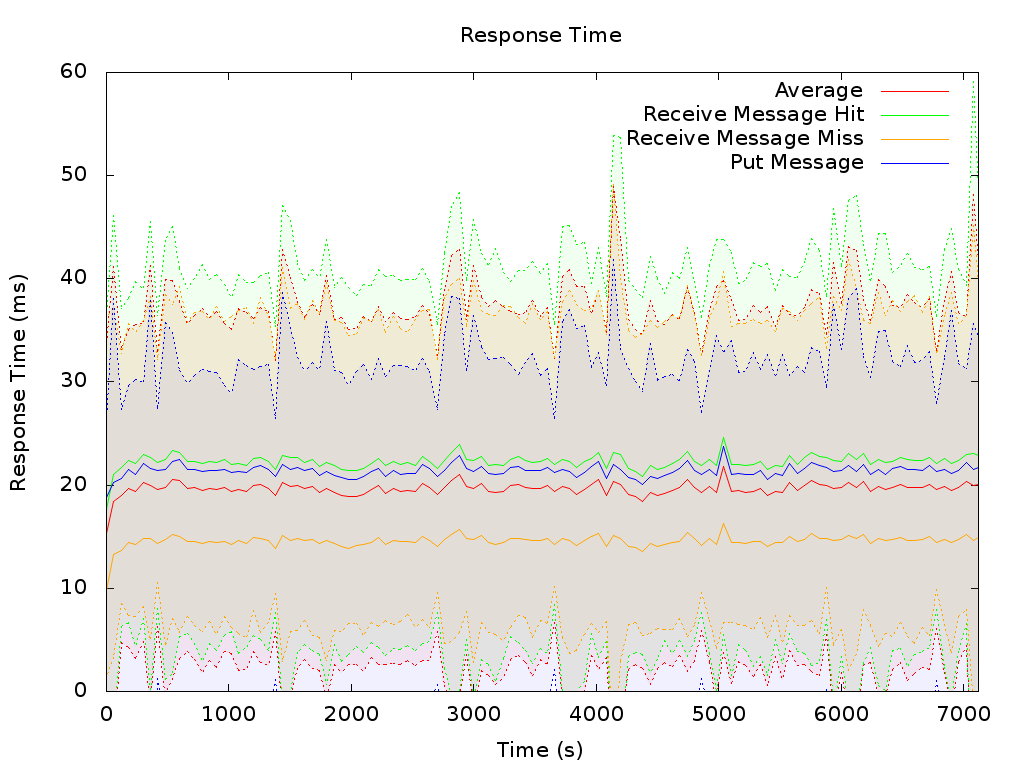
\includegraphics[width=0.9\textwidth]{graphs/response-time}
        \caption{Middleware response time for different request types, averaged over an interval of one minute.}
        \label{fig:response-time}
    \end{figure}
    
	\Cref{fig:response-time} shows the middleware response time as measured by the clients over time.
	The response time is averaged over the interval of one minute for each of the shown curves.
	
	The averaged middleware response time seems fairly stable over long periods of time, the individual
	measurements however fluctuate quite heavily as can be seen by the relatively large standard deviation.
	This effect is not very concerning as the absolute value of the standard deviation (generally less than
	25ms) is quite small and can easily be caused by interference of other tasks run on the same physical
	machine.
	
	The different types of requests take roughly the same time to complete, message request misses being
	slightly faster than the rest. This is caused directly by the way the database operates, it neither has
	to write or read any complex data as the necessary information is already available in the index. 
	
	\begin{figure}[ht]
    \centering
        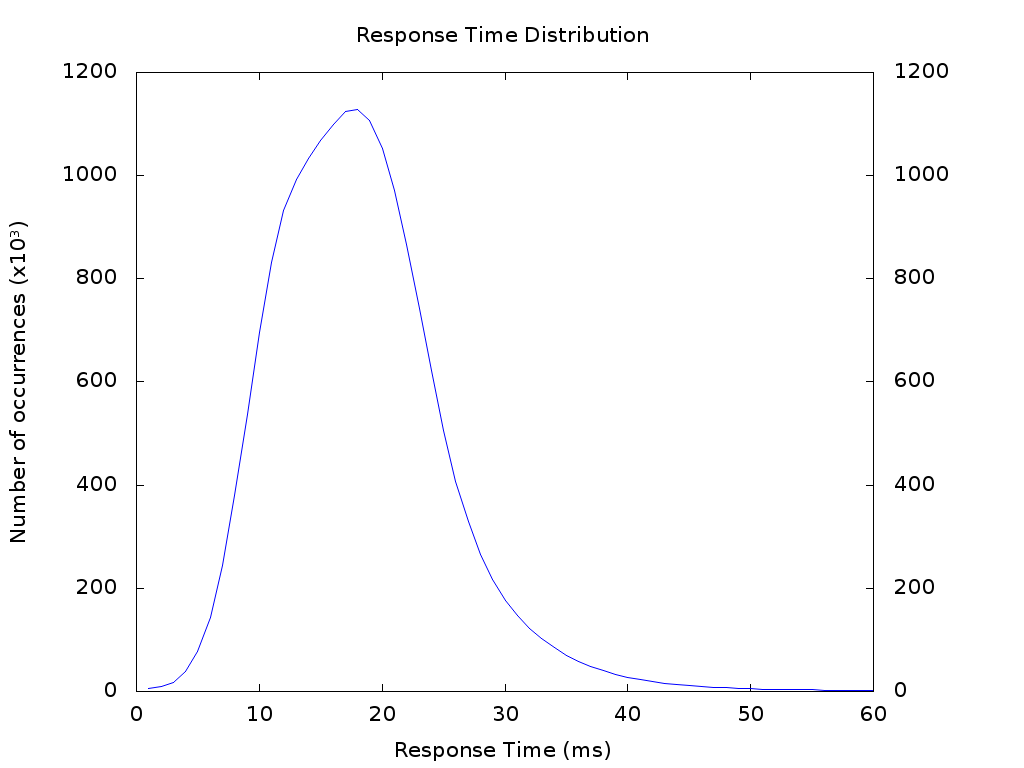
\includegraphics[width=0.9\textwidth]{graphs/distribution}
        \caption{Middleware response time distribution measured in chunks of 1 millisecond.}
        \label{fig:distribution}
    \end{figure}
    
    \Cref{fig:distribution} shows the distribution of the observed middleware response time during
    the two hour long experiment. As expected it roughly follows a normal distribution with no
    values being higher than one second.

\subsection{Benchmarks}
	\begin{table}[hp]
        \centering
        \rowcolors{1}{Gray}{white}
        \begin{tabular}{$l^c^r}
            \rowcolor{DarkGray}
            \rowstyle{\bfseries}
            Phase & Time & Relative\\
            \hline
            Waiting for client & \SI{79}{\micro\second} & 0.82\%\\
            Parsing request & \SI{14}{\micro\second} & 0.15\%\\    
            Waiting for database & \SI{9,574}{\micro\second} & 98.80\%\\
            Responding & \SI{22}{\micro\second} & 0.23\%\\       
        \end{tabular}
        \caption{Time spent on various tasks by middleware workers}
        \label{tbl:benchmark}
    \end{table}
    
    \Cref{tbl:benchmark} shows the time spent by the middleware on various tasks while handline a
    request. It is clearly visible that most of the time, over 98\%, is spent waiting for the database.
    From \cref{fig:response-time} we can also conclude that around half of the time a request takes is
    spent by the middleware and the other half is needed for networking.

\newpage
\subsection{Scalability}
	We conducted various experiments to figure out the optimal parameters for the system and see how
	well it scales with higher load.

\subsubsection{Worker Thread Count}
    \begin{figure}[ht]
    \centering
        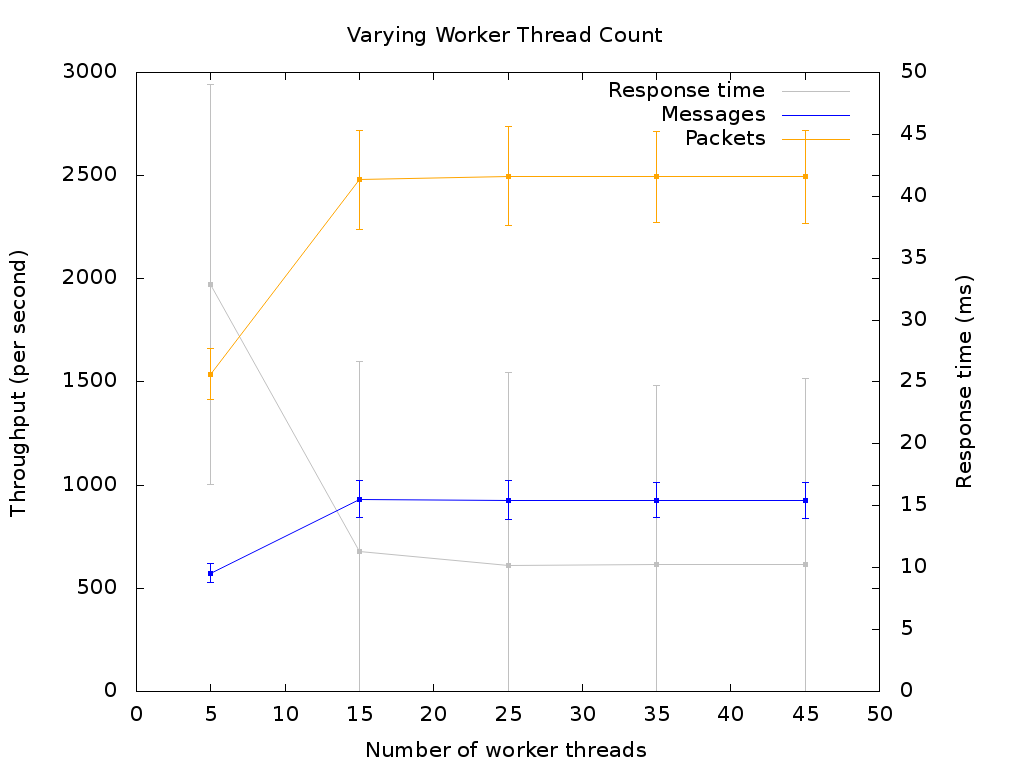
\includegraphics[width=0.9\textwidth]{graphs/worker}
        \caption{Throughput and response time for varying number of worker instances}
        \label{fig:worker}
    \end{figure}
    
    \Cref{fig:worker} shows the system with a varying number of worker threads but the same
    number of database connections (25). It can be seen that increasing the worker thread count beyond
    the number of database connections clearly doesn't increase throughput, it can even be lowered and
    the system performs equally well.

\newpage
\subsubsection{Database Connection Count}
    \begin{figure}[ht]
    \centering
        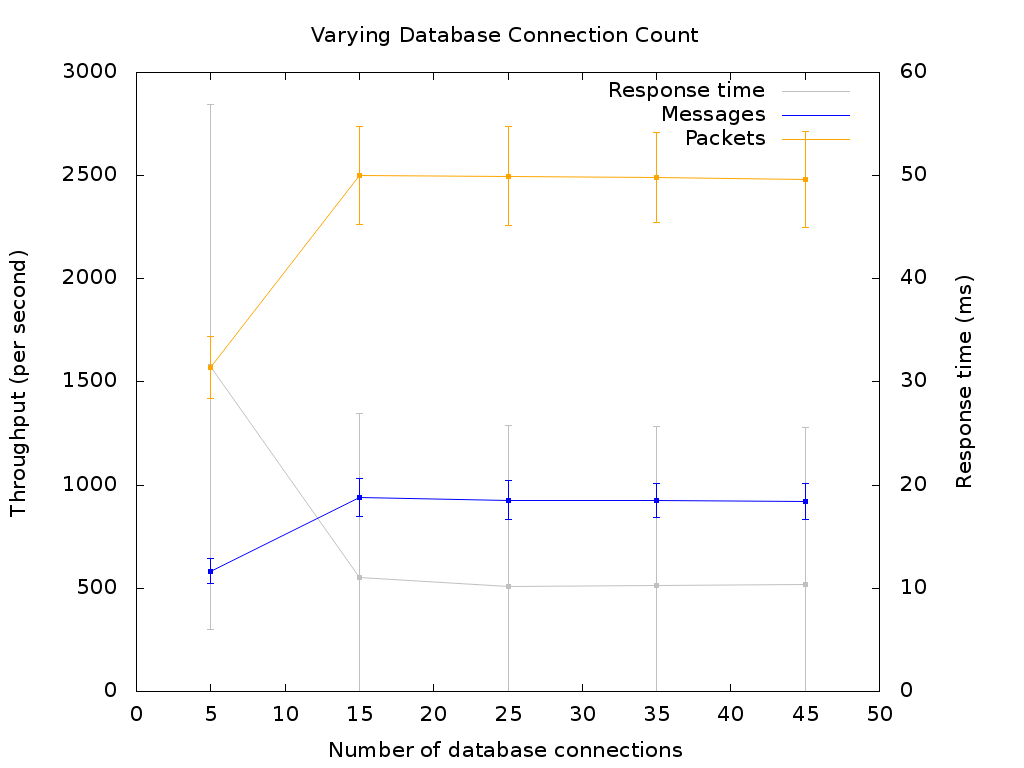
\includegraphics[width=0.9\textwidth]{graphs/db}
        \caption{Throughput and response time for varying number of database connections}
        \label{fig:db}
    \end{figure}
    
    \Cref{fig:db} shows the performance of the system with various numbers of database connections and
    a static number of worker threads (25). It can again be seen that the optimal performance is already
    reached with only 15 connections. The fact that the performance doesn't increase until the number
    of worker threads is reached shows that the database can in fact not process requests any faster
    than our middleware is able to send over 15 connections.

\newpage
\subsubsection{Combined Database Connection and Worker Thread count}
    \begin{figure}[ht]
    \centering
        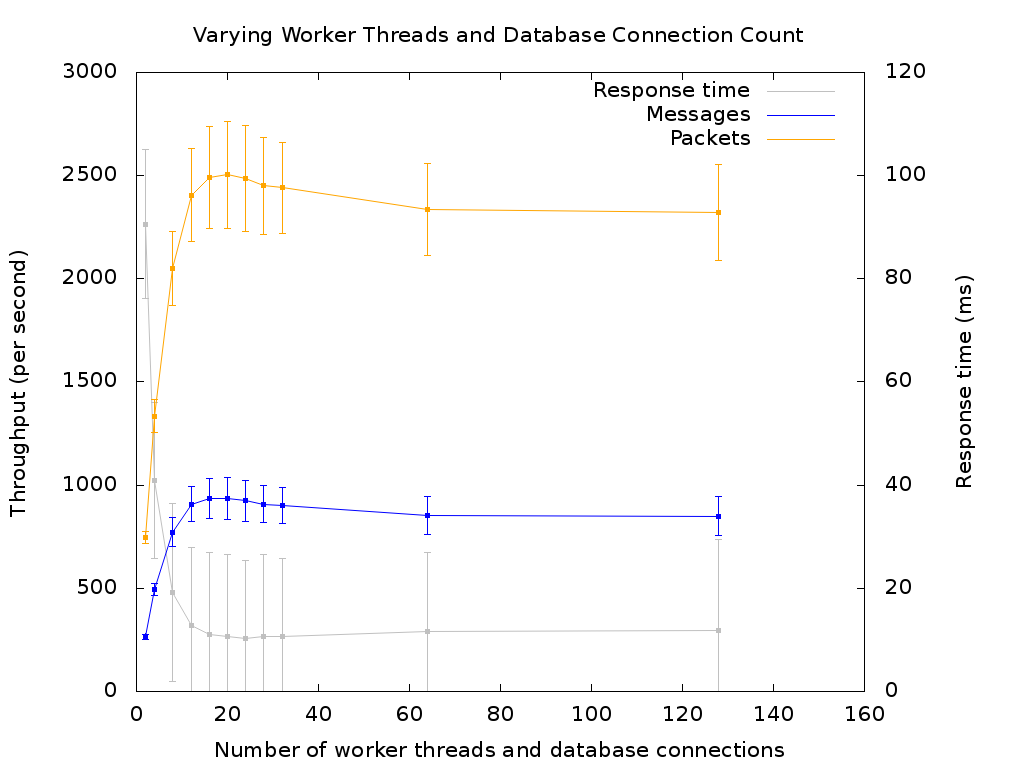
\includegraphics[width=0.9\textwidth]{graphs/db+worker}
        \caption{Throughput and response time for varying number of worker instances and database connections}
        \label{fig:db+worker}
    \end{figure}
    
    Since worker thread and database connection count seem to be linked we increased them together as shown in
    \cref{fig:db+worker}. Again, the best performance is achieved around a value of 20 and it decreases
    slowly as more workers and connections are added. The steep slope to the left of the optimal value
    is the range where the database still has free resources and the middleware can't make requests
    fast enough. 

\newpage
\subsubsection{Client Retry Delay}
    \begin{figure}[ht]
    \centering
        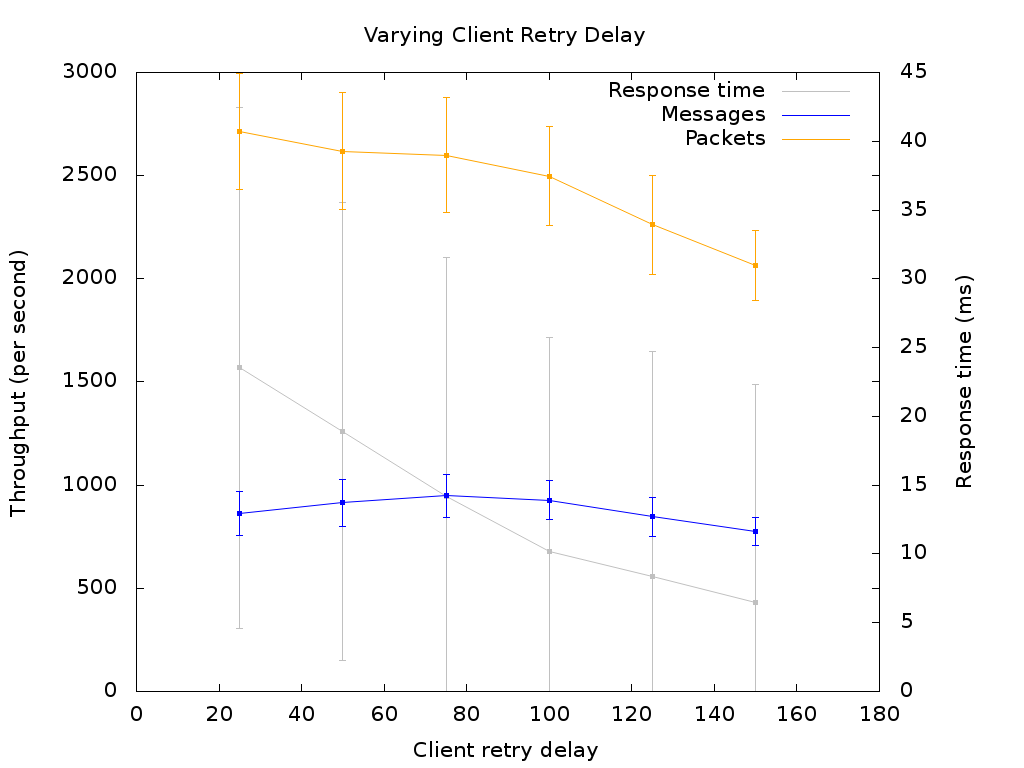
\includegraphics[width=0.9\textwidth]{graphs/client-delay}
        \caption{Throughput and response time for varying client retry delay}
        \label{fig:client-delay}
    \end{figure}
    
    In this experiment we varied the amount of time a client waits before retrying to retrieve a message.
    As seen in \cref{fig:client-delay} this parameter doesn't have a very huge impact on the message throughput
    of the system, it does however decreases the overall packet count (and therefore throughput) because
    less packets are wasted when querying for nonexisting messages. A higher retry delay also causes the
    average response time to decrease as the middleware can process the lower number of packets much faster.
    The ideal value in regard to message throughput appears to be between 80 and \SI{100}{\milli\second}.

\newpage
\subsubsection{Client Count}
    \begin{figure}[ht]
    \centering
        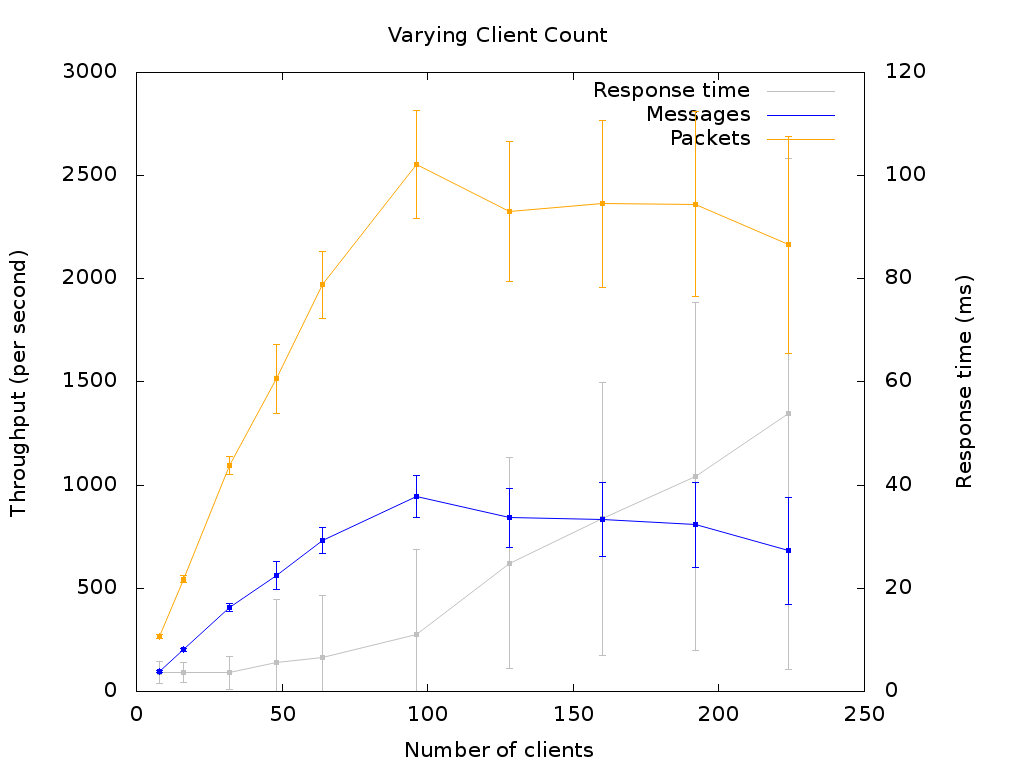
\includegraphics[width=0.9\textwidth]{graphs/client}
        \caption{Throughput and response time for varying number of clients}
        \label{fig:client}
    \end{figure}
    
    When running the system with an increased number of clients we noticed a small but clear drop in 
    message throughput as can be seen in the right half of \cref{fig:client}. When using less clients
    than the usual 90 the system was underloaded which also resulted in much lower throughput of both
    messages and network packets. The response time steadily rises with the growing number of clients
    as expected. It's also noticeable how the system behaves much more predictably while underloaded
    than overloaded as can be seen by the very small standard deviation for low numbers of clients.
    
\newpage
\subsubsection{Middleware Count}
    \begin{figure}[ht]
    \centering
        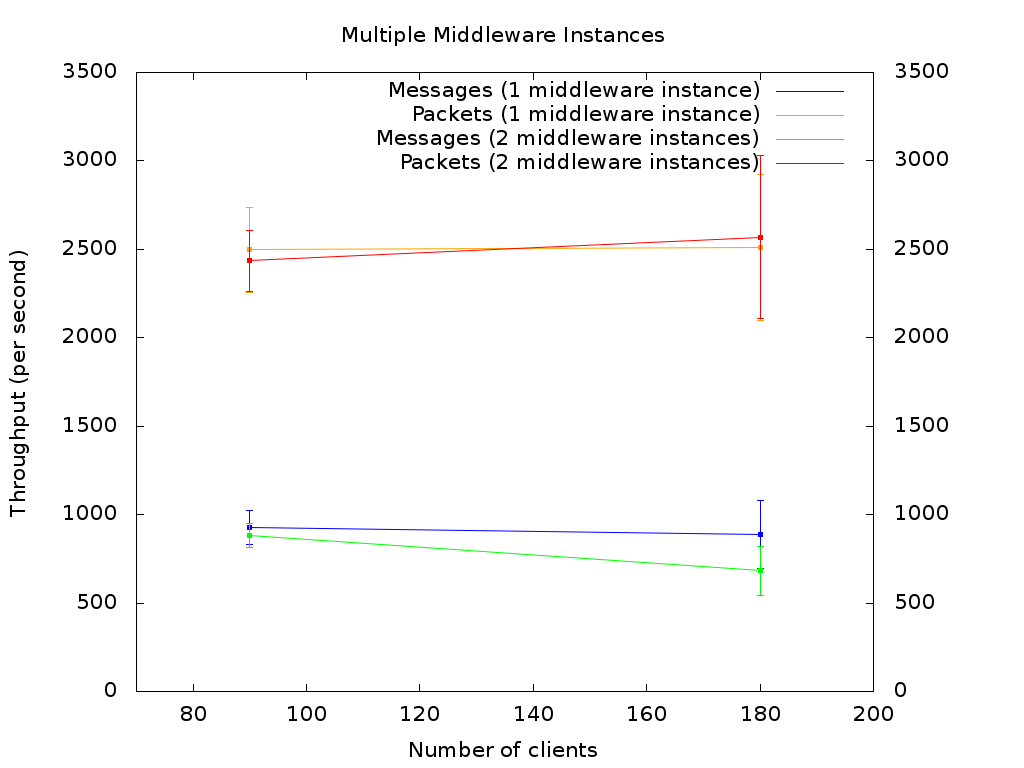
\includegraphics[width=0.9\textwidth]{graphs/multi}
        \caption{Throughput and response time for varying number of clients with both one and two middleware instances}
        \label{fig:multi}
    \end{figure}
    
    We conducted most of our experiments on a single middleware instance as it was already evident
    that not the middleware but the database was limiting the system performance. The two measurements
    shown in \cref{fig:multi} proof that adding more middleware instances does indeed not improve
    performance. The second middleware was run on the same {\it EC2} instance as the first one, but
    we payed close attention to the usage of memory, CPU and the network to make sure they wouldn't
    interfere with each other.
    

\chapter{Conclusion}
    As discussed in \cref{ch:evaluation}, the major bottleneck in the
    performance of \telesto{} is the database. It is important to note, that we
    did no experiments to optimize the database configuration. Most likely a
    more optimal configuration of the database would have improved the overall
    performance of the system but when looking at the relative time consumption
    for tasks by middleware workers (\cref{tbl:benchmark}) it is very unlikely
    that an other part would actually become the new bottleneck.
	
	When looking at the completed \telesto{} implementation we are confident to
	have built a scalable and well performing distributed message passing
	system that fulfils the given requirements. The number of tests and traces with
	different metrics we executed, is sufficient to allow for reasonable
	conclusions and optimization of the most important system and workload
	parameters.
	
	In the end we learned a lot about testing and benchmarking an entire system in
	a profound way and drawing comprehensible conclusions. Although both of us
	already had experience in building a large system from scratch, we got a lot of
	interesting insights in how it could look like when building and especially
	evaluating a system in the industry which might not even be that far away...
	

% This displays the bibliography for all cited external documents. All references have to be defined in the file references.bib and can then be cited from within this document.
\bibliographystyle{splncs}
\bibliography{references}

% This creates an appendix chapter, comment if not needed.
%\appendix
%\chapter{Appendix Chapter}

%\section{Database Structure}

	
\end{document}